\chapter{DESENVOLVIMENTO}
\label{c.Desenvolvimento}

O desenvolvimento do projeto dividiu-se em quatro fases: a montagem do ambiente de testes de assinaturas construídas
a partir de regras do Yara; a obtenção das regras e construção de um índice de agrupamento das mesmas para agilizar a
execução das varreduras; obtenção e escolha de amostras de \textit{malware} para testagem; bateria de testes final e
análise de resultados. Complementarmente, foi desenvolvida a ideia de uma aplicação \textit{web} para análise
de \textit{malware} com base em regras de detecção do Yara.

\section{Obtenção das regras de detecção e das amostras de \textit{malware}}
\label{s.obtregras}

A primeira etapa da implementação computacional do projeto foi a construção de um índice de regras do Yara compilado a partir das
bases de assinaturas do ClamAV e de outros conjuntos avulsos e menores de assinaturas disponibilizados em repositórios de código
aberto; em paralelo, também construiu-se um conjunto de algumas amostras vivas e selecionadas de \textit{malware} para a testagem
do índice sobre arquivos infectados. Foram selecionadas apenas amostras de \textit{malware} `potencialmente inofensivo', como
\textit{trojans}, que dependem de um comando de execução disparado por um usuário descuidado, para que não houvesse risco de
propagação e infecção do próprio ambiente local e de redes com as quais o ambiente local se comunicasse. Por isso, com fins de
prevenção, optou-se pela não realização de testes em, por exemplo, \textit{worms}, que conseguem se propagar de maneira independente
pelos ambientes onde chegam. Para converter as assinaturas, foi adaptado um \textit{script} em Python que interpreta os arquivos no
que contém as assinaturas do ClamAV, cujo formato é .cvd, e reescreve-as na sintaxe amigável de regras do Yara. No final da seção
de desenvolvimento, há uma lista com os \textit{links} para \textit{download} de todo o código-fonte do projeto. Após a tradução
das regras contidas nas bases de dados, é necessário compilá-las antes de finalmente ser possível aplicá-las numa varredura
real. Um outro pequeno \textit{script} em Python é capaz de realizar essa tarefa, vide código-fonte exibido na figura abaixo:
\begin{figure}
  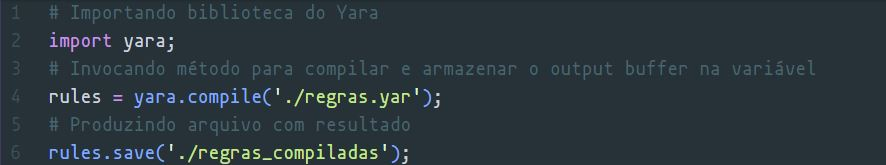
\includegraphics[scale=0.6]{figs/script_conversao}
  \centering
  \caption{Script para compilação das regras de detecção}
  \label{f.script_comp}
\end{figure}


\section{Testes iniciais com o ambiente de desenvolvimento}
\label{s.testesiniciais}

\section{Testagem completa e análise de resultados}
\label{s.testefull}

\section{Ideia de uma aplicação web do projeto desenvolvido}
\label{s.prototipo}

Foi elaborada a ideia de um serviço capaz de receber regras do Yara ou arquivos de bases de assinaturas de \textit{malware}
para manter sua própria base de dados unificada e também capaz de realizar varreduras em arquivos carregados pelos usuários
ao servidor da aplicação. Na imagem a seguir temos um esboço do funcionamento da aplicação projetada.

\begin{figure}[H]
  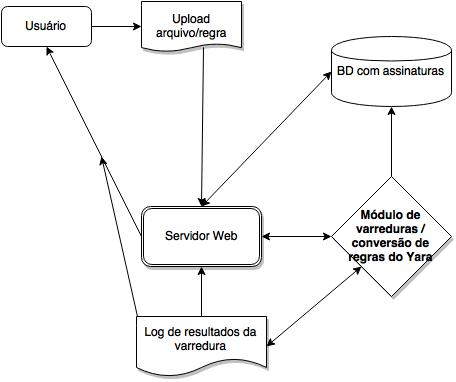
\includegraphics[scale=0.6]{figs/flux_prototipo}
  \centering
  \caption{Fluxograma de funcionamento da aplicação. Fonte: elaborada pelo autor.}
  \label{f.flux_prototipo}
\end{figure}
% TODO
% Listar estrutura de pastas do módulo de conversão e varredura
% Detalhar o funcionamento do desgraçado
% Mostrar o front-end e explicar como funcionaria o backend
% Escrever a conclusão
% Mandar para o Kelton Revisar
% Rezar para os deuses do TCC me olharem com bondade
% Comprar 5 fardos de cerveja
% 2 KG de carne
% 50g de aipim jamaicano
% Party hard.
